\section{Serie Temporali | Time Series}
\label{sec:time-series}

Le serie temporali vengono usate in campi come la \textbf{predizione di prezzi
    di azioni}, che richiedono una conoscenza dei trend passati per funzionare. Le
reti neurali Feed Forward non considerano gli stati temporali. Si utilizza,
infatti, un'altra architettura di rete neurale: \textbf{Recurrent Network -
    RNN}

\subsection{Recurrent Neural Network RNN}

Una RNN itera sugli elementi mantenendo uno stato che contiene informazioni di
ciò che è stato visto finora. Questo stato viene passato avanti ad ogni
iterazione.

\begin{definition} RNN

\end{definition}

Una RNN è un grafo con cicli. I percettroni beneficiano del feedback dei loop.
L'output di un percettrone al tempo $t$ è coinvolto nel calcolo dell'output di
un percettrone al tempo $t+1$.

%figura da fare
\begin{figure}[H]
    \begin{center}
        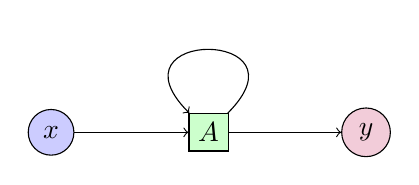
\begin{tikzpicture}
            \node[fill=blue!20, draw,circle] (x) at (0,0) {$x$};
            \node[fill=green!20, draw,rectangle] (A) at (2,0) {$A$};
            \node[fill=purple!20, draw,circle] (y) at (4,0) {$y$};
            \draw[->] (x) -- (A);
            \draw[->] (A) -- (y);
            \draw[->] (A) to [out=45,in=135,looseness=8] (A);
        \end{tikzpicture}
    \end{center}
    \caption{RNN}
\end{figure}

%figura da fare
\begin{figure}[H]
    \begin{center}
        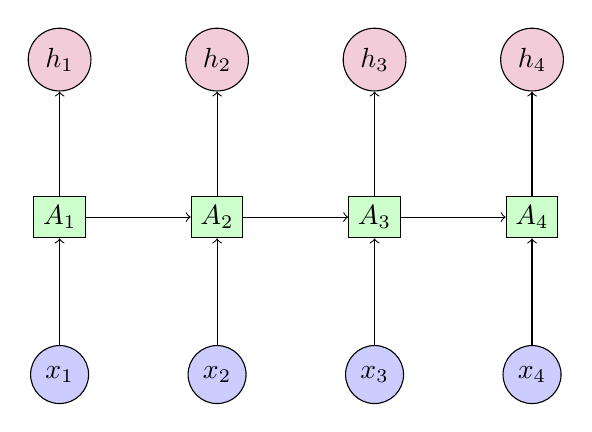
\begin{tikzpicture}
            \node[fill=blue!20, draw,circle] (x_1) at (0,0) {$x_1$};
            \node[fill=green!20, draw,rectangle] (A_1) at (0,2) {$A_1$};
            \node[fill=purple!20,draw,circle] (y_1) at (0,4) {$h_1$};

            \node[fill=blue!20, draw,circle] (x_2) at (2,0) {$x_2$};
            \node[fill=green!20, draw,rectangle] (A_2) at (2,2) {$A_2$};
            \node[fill=purple!20,draw,circle] (y_2) at (2,4) {$h_2$};

            \node[fill=blue!20, draw,circle] (x_3) at (4,0) {$x_3$};
            \node[fill=green!20, draw,rectangle] (A_3) at (4,2) {$A_3$};
            \node[fill=purple!20,draw,circle] (y_3) at (4,4) {$h_3$};

            \node[fill=blue!20, draw,circle] (x_4) at (6,0) {$x_4$};
            \node[fill=green!20, draw,rectangle] (A_4) at (6,2) {$A_4$};
            \node[fill=purple!20,draw,circle] (y_4) at (6,4) {$h_4$};

            \draw[->] (x_1) -- (A_1);
            \draw[->] (A_1) -- (y_1);

            \draw[->] (x_2) -- (A_2);
            \draw[->] (A_2) -- (y_2);

            \draw[->] (x_3) -- (A_3);
            \draw[->] (A_3) -- (y_3);

            \draw[->] (x_4) -- (A_4);
            \draw[->] (A_4) -- (y_4);

            \draw[->] (A_1) -- (A_2);
            \draw[->] (A_2) -- (A_3);
            \draw[->] (A_3) -- (A_4);
        \end{tikzpicture}
    \end{center}
    \caption{Unfolded RNN}
\end{figure}

\textbf{Ci sono 2 equazioni da tenere a mente}:

\textbf{Rete Elman:}
\begin{equation}
    \begin{aligned}
        h_t = \sigma(W_h x_t + U_h \textcolor{green}{h_{t-1}}+b_h) \\
        y_t = \sigma(W_y h_t + b_y)
    \end{aligned}
\end{equation}

\textbf{Rete Jordan:}
\begin{equation}
    \begin{aligned}
        h_t = \sigma(W_h x_t + U_h \textcolor{purple}{y_{t-1}}+b_h) \\
        y_t = \sigma(W_y h_t + b_y)
    \end{aligned}
\end{equation}

Dove:
\begin{itemize}
    \item $x_t$ = Vettore di input
    \item $y_t$ = Vettore di output
    \item $h_t$ = Vettore di layer nascosto
    \item $W,U,b$ = Pesi e Bias
    \item $\sigma_h, \sigma_y$ = Funzioni di attivazione
\end{itemize}

%inserisci foto
\begin{figure}
    \begin{center}
        \includegraphics[scale=0.8]{images/RNN.png}
    \end{center}
    \caption{RNN}
\end{figure}

\subsubsection{L'utilizzo delle RNN}

Alla fine, tutto ciò che noi andiamo a fare è \textbf{aggiungere dei layer}
alla nostra rete.

\begin{lstlisting}[language=python]
    model.add(SimpleRNN(32, return_sequences=True))#Return a list
    model.add(SimpleRNN(32, return_sequences=True))#Return a list
    model.add(SimpleRNN(32, return_sequences=True))#Return a list
    model.add(SimpleRNN(32)) # last layer only returns last output

    model.summary()
\end{lstlisting}

Un esempio di codice di rete è:

\begin{lstlisting}[language=python]
from keras.datasets import imdb
from keras.preprocessing import sequence

max_features = 10000 # number of words to consider as features
maxlen = 500
batch_size = 32

(input_train, y_train), (input_test, y_test) = imdb.load_data(num_words=max_features)

input_train = sequence.pad_sequences(input_train, maxlen=maxlen)
input_test = sequence.pad_sequences(input_test, maxlen=maxlen)

from keras.layers import Dense

model = Sequential()
model.add(Embedding(max_features, 32))
model.add(SimpleRNN(16))
model.add(Dense(1, activation='sigmoid'))
model.compile(optimizer='rmsprop'
            , loss='binary_crossentropy'
            , metrics=['acc'])

history = model.fit(input_train, y_train,
            epochs=10,
            batch_size=128,
            validation_split=0.2)
\end{lstlisting}

Questo codice ha un problema: \textbf{non funziona}. Il problema è la
\textbf{back propagation} attraverso il tempo. La normale backpropagation non
funziona e ha bisogno di un cambiamento per adattarsi al \textbf{feedback
    loop}. Immaginiamo di avere una funzione del genere:
\begin{equation}
    f(f(f(f(f(f(f(f(f(f(f(f(x_0 | x_1 , \dots , x_n))))))))))))
\end{equation}

Praticamente si ha un numero di derivate ripetuto. Poi, dalle slides, dopo
tutti i calcoli si arriva ad avere un risultato in cui la derivata ha valore
che \textbf{tende sempre a 0}. Come se si trovasse sempre un minimo globale.
Quindi, questo approccio non funziona. Il \textbf{gradiente sparisce}

\textbf{Motivazione:} la sequenza è troppo lunga.
\begin{definition}(
    Spiegazione del problema )

    Il problema della dipendenza a lungo termine è una sfida nell'addestramento
    delle reti neurali artificiali, in particolare le reti neurali ricorrenti
    (RNN). Si riferisce alla difficoltà che queste reti hanno nell'apprendere a
    collegare informazioni o contesti da passaggi precedenti nella sequenza a
    passaggi successivi.

    Ad esempio, considera un modello di linguaggio che cerca di prevedere la parola
    successiva in una frase. Se la frase è "Sono cresciuto in Francia... parlo
    fluentemente ---", il modello deve ricordare il contesto della "Francia" da
    molto prima nella frase quando arriva al punto vuoto, così può riempirlo con
    "francese". Questa è una dipendenza a lungo termine.

    Le RNN fanno fatica con questo a causa del problema dei "gradienti che
    svaniscono". Durante la retropropagazione, i gradienti spesso diventano sempre
    più piccoli man mano che vengono propagati all'indietro nel tempo. Ciò
    significa che gli aggiornamenti ai pesi che collegano i passaggi precedenti
    nella sequenza a quelli successivi possono essere molto piccoli, e la rete può
    non riuscire a imparare queste dipendenze a lungo termine.
\end{definition}

Una proposta di soluzione è quella di \textbf{cambiare la funzione di
    attivazione}.

\textbf{Soluzione}: Long Short Term Memory (LSTM)

\subsection{Long Short Term Memory (LSTM)}

Queste RNN speciali sono reti capaci di risolvere il problema delle dipendenze
a lungo termine. In paticolare, sono state progettate per \textbf{controllare
    la sparizione del gradiente} e \textbf{evitare proprio il problema della
    dipendenza a lungo termine}

%inserisci foto
\begin{figure}
    \begin{center}
        \includegraphics[scale=0.8]{images/LSTM.png}
    \end{center}
    \caption{LSTM}
\end{figure}
Riguardo l'archiettura, parliamo di una cosa importante.

\textbf{Lo stato della cella} salva un'informazione interna della catena \textbf{Storico interno}. Questa informazione,
se rilevante, può essere \textbf{propagata}. Per controllare il flow di queste informazioni si una un \textbf{gate}. Servono, appunto,
per decidere quali informazioni far passare.

\textbf{Ci sono formule da ricopiare}
\begin{itemize}
    \item \textbf{Forget Gate}: decide quali informazioni scartare e quali tenere
          \[
              f_t = \sigma(W_f \cdot[h_{t-1}, x_t] + b_f)\]
          \begin{figure}[H]
              \begin{center}
                  \includegraphics[scale=0.8]{images/forgetgate.png}
              \end{center}
              \caption{Forget Gate}
          \end{figure}
    \item \textbf{Input Gate}: decide quali informazioni passare e quanto devono influenzare lo storico interno
          \begin{equation}
              \begin{aligned}
                  i_t = \sigma(W_i \cdot [h_{t-1}, x_t] + b_1)       \\
                  \tilde{C}_t = tanh(W_C \cdot [h_{t-1}, x_t] + b_C) \\
              \end{aligned}
          \end{equation}
          \begin{figure}[H]
              \begin{center}
                  \includegraphics[scale=0.8]{images/inputgate.png}
              \end{center}
              \caption{Input Gate}
          \end{figure}
    \item \textbf{Aggiornamento dello stato interno}: Gate che risolvono il problema della dipendenza a lungo termine e del gradiente che svanisce
          \[
              C_t = f_t * C_{t-1} + i_t * \tilde{C_t}\]
          \begin{figure}[H]
              \begin{center}
                  \includegraphics[scale=0.8]{images/update.png}
              \end{center}
              \caption{Update State}
          \end{figure}
    \item \textbf{Output Gate}: L'output dipende dallo stato interno della cella. La LSTM controlla quanto l'output deve essere influenzato dallo storico interno
          \begin{equation}
              \begin{aligned}
                  o_t = \sigma(W_o \cdot [h_{t-1}, x_t] + b_o) \\
                  h_t = o_t * tanh(C_t)
              \end{aligned}
          \end{equation}
          \begin{figure}[H]
              \begin{center}
                  \includegraphics[scale=0.8]{images/outputgate.png}
              \end{center}
              \caption{Output Gate}
          \end{figure}

\end{itemize}

Ricordiamo che gli elementi sono:
\begin{itemize}
    \item $x_t$ = Vettore di input
    \item $y_t$ = Vettore di output
    \item $h_t$ = Vettore di layer nascosto
    \item $W,U,b$ = Pesi e Bias
    \item $\sigma_h, \sigma_y$ = Funzioni di attivazione
\end{itemize}

\begin{lstlisting}[language=python]
from keras.layers import LSTM

model = Sequential()
model.add(Embedding(max_features, 32))
model.add(LSTM(32))
model.add(Dense(1, activation='sigmoid'))
model.compile(optimizer='rmsprop'
            ,loss='binary_crossentropy'
            ,metrics=['acc'])

            history = model.fit(input_train, y_train,
epochs=10,
batch_size=128,
validation_split=0.2)
\end{lstlisting}

\newpage